\vspace{10pt}

{\centering\subsection*{周璇:如何描写人物?}}

\addcontentsline{toc}{subsection}{周璇:如何描写人物?}

\renewcommand{\leftmark}{周璇:如何描写人物?}

\begin{figure}[htbp]

\centering

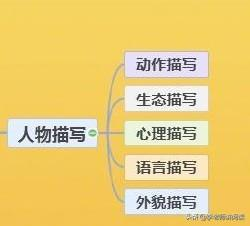
\includegraphics[width = .5\textwidth]{./ch/v4.jpg}

\end{figure}


与你共同成长。



你好,这里是桂花图书馆写作分享,我是馆长莫静琴。



这一周,我们邀请到柏墩小学五二班的语文老师周璇老师来与大家分享如何进行人物描写。有什么方法可以让笔下的人物生动、形象而真实呢?我们一起来听听周老师的分享。





人物描写是小学中高年级段的习作侧重点。这就要求教师在日常的课文教学和单独的习作教学中,将重心放在“如何进行人物描写”上。



首先,我们要理清一个思路。人物描写,不仅仅是人物外貌的描写。



我们在描写某一个人物时,通常是要通过一系列的描写手法来体会这个人物的内心和性格特点,仅仅一个外貌描写完全不足以达到我们的写作目的。



其次,我们要理解三个方面。



进行人物描写的习作时,我们究竟怎样才能通过文字展现一个人呢?我认为有以下三个方面:



一是正面描写。所谓正面描写,就是直接描写人物的外貌、神态、心理、动作和语言,把人物的状态直接具体地描绘出来。



二是侧面描写。侧面描写则是指作者通过对周围人物或环境的描绘来表现所要描写的某个人物。



三是具体事例的叙述。我们对人物的语言、神态等各方面的描述,都是要在具体事件中体现的。将各种方面的描写融入进某一件或某几件事情中,才能体现人物的某些特点。只有这人三方面的融合,才能达到我们进行人物习作的目的。



最后,我们要坚持一个理念。“感人心者莫过于情”。



人物描写的习作,一般都以记叙文的形式呈现出来。我们通常都是通过一篇习作,体现自己对某个人的深刻认识,或者表达自己从这个人身上学到知识后的感想。所以,这类作文最重要的一个技巧就是抒发真情实感。只有真实,才能使作文中的人物更具生命力。如果全篇的虚情假意或者无中生有,只会让人读起来了无乐趣。





分享听完了。从周老师的分享中,我们了解到:



人物描写要外貌描写和心理描写相结合。



除了正面描写外,还可以进行侧面的和具体事例的描写,在真情实感的基础上,对人物进行立体的刻画。



好了,这周的分享就到这里。愿大家五一假期平安顺利!




\vspace{10pt}


作者:周璇

朗读:周璇

发布:2021年5月1日







\vspace{10pt}

\hline

